\documentclass{article}
\usepackage{graphicx} % Graficas.
\usepackage[utf8]{inputenc} % Uso de UTF.
\usepackage[hidelinks]{hyperref} % Indice con hipervinculos.
\usepackage{caption}
\usepackage{listings} % Copeo de codigo.
\usepackage{fullpage} % Uso de pagina completa.
\usepackage{color} % Color para codigo.
\renewcommand*\contentsname{Indice}

\begin{document}

\begin{figure}[!htb]
\minipage{0.32\textwidth}
	\includegraphics[width=\linewidth]{"img/LogoSEP".png}
\endminipage\hfill
\minipage{0.32\textwidth}
	\includegraphics[width=\linewidth]{"img/LogoTNM".PNG}
\endminipage\hfill
\minipage{0.32\textwidth}
	\includegraphics[width=\linewidth]{"img/LogoITT".png}
\endminipage\hfill
\end{figure}

\begingroup
\LARGE
\begin{verbatim}
Subdireccion Academica
Departamento de Sistemas y Computacion
Ingenieria en Sistemas Computacionales
Semestre: Enero - Junio 2017
Materia: Sistemas Programables (3SC8A)

Nombre del tema:
Documentacion proyecto

Nombre de los integrantes:
Salcedo Morales Jose Manuel (13211419)
Espinoza Covarrubias Silverio Alejandro (13211465)
Álvarez Corral Miguel Ángel (13211384)

Nombre del catedratico:
Ingeniero Luis Alberto Mitre Padilla

\end{verbatim}
\endgroup

\newpage
\tableofcontents

\newpage
\section{Introduccion}

\section{Componentes utilizados}
\begin{itemize}
        \item Arduino
        \item Cables Jumper
        \item Fuente de alimentacion para arduino
\end{itemize}

\newpage
\section{Marco Teorico}
\begin{itemize}
	\item Arduino: Arduino se refiere a una plataforma o placa de electronica de codigo abierto y al software utilizado para programarlo. Arduino esta diseñado para hacer la electronica mas accesible a los artistas, diseñadores, aficionados y a cualquiera interesado en la creacion de objetos interactivos o entornos. Un tablero de Arduino se puede comprar pre-ensamblado o, porque el diseño de hardware es de codigo abierto, construido a mano. De cualquier manera, los usuarios pueden adaptar las tablas a sus necesidades, asi como actualizar y distribuir sus propias versiones.
\end{itemize}

Este proyecto ha sido realizado con los siguientes componenetes:

\begin{itemize}
	\item Arduino UNO
	\item Protoboard
	\item Sensor de humedad en suelo
	\item Sensor de humedad  y temperatura (DTH11)
	\item Sensor barometrico BMP180
	\item Fotorresistencia
	\item Relay 5VDC – 120 VAC
	\item Resistencia
	\item Diodo 1N4007
\end{itemize}

\subsection{Arduino UNO}

El Arduino Uno es una placa electronica basada en el  ATmega328  (ficha tecnica). Cuenta con 14 pines digitales de entrada / salida (de los cuales 6 se pueden utilizar como salidas PWM), 6 entradas analogicas, un 16  MHz  resonador de ceramica, de una conexion USB, un conector de alimentacion, una cabecera ICSP, y un boton de reinicio.

\subsection{Protoboard}

Es una especia de tablero con orificios, en la cual se pueden insertar componentes electronicos y cables para armar circuitos. Como su nombre lo indica, esta tableta sirve para experimentar con circuitos electronicos, con lo que se asegura un buen funcionamiento del mismo. 

\subsection{Sensor de humedad en suelo}

Este sensor de humedad puede leer la cantidad de humedad presente en el suelo que lo rodea. Es un sensor de baja tecnologia, pero es ideal para el seguimiento de un jardin urbano. Se trata de una herramienta indispensable para un jardin de contacto.

Este sensor utiliza las dos sondas para pasar corriente a traves del suelo, y luego  lee la resistencia para obtener el nivel de humedad. Mas agua hace que el suelo conduzca la electricidad con mayor facilidad (menos resistencia), mientras que el suelo seco es un mal conductor de la electricidad (mas resistencia).

Caracteristicas:

\begin{itemize}
	\item Sensibilidad ajustable ajustando el potenciometro digital (azul).
	\item Voltaje de operacion: 3.3V ~ 5V
	\item Modo de salida dual, salida digital y salida analogica mas precisa.
	\item Agujeros de montaje para una facil instalacion.
	\item Dimensiones PCB: 30mm * 16mm.
	\item Dimensiones de sonda: 60mm * 30mm.
	\item Indicador de energia. Indicador alimentacion (rojo) e indicador de salida de conmutacion digital (verde).
	\item El modulo tiene un amplificador LM393.
\end{itemize}

Defnicion de pines:

\begin{itemize}
	\item VCC (5V)
	\item GND
	\item Interfaz de salida digital (0 y 1) 
	\item Interfaz de salida analogica AO
\end{itemize}

\subsection{Sensor de humedad  y temperatura (DTH11)}
Tarjeta con Sensor DHT11 Humedad resistivo ideal para sistemas de medicion climatologicos o para controles de temperatura y humedad. Este sensor ademas incluye un sensor interno de temperatura NTC. Este modulo tiene una gran relacion señal a ruido ante la interferencia y es muy durable.
Especificaciones:

\begin{itemize}
	\item Sensor resistivo de humedad
	\item Sensor de temperatura NTC
	\item Voltaje de alimentacion: 5V
	\item Rango de temperatura: 0-50ºC
	\item Rango de humedad: 20-90{\%}RH
	\item Tamaño: 25 x 16 x 7 mm
	\item Peso: 9g
\end{itemize}


\subsection{Sensor barometrico BMP180}

Ésta placa incluye un sensor de presion barometrica BMP180 de alta precision con un rango de medida de entre 300 y 1100 hPa (Hecto Pascal) con un margen de error minimo de tan solo 0.03 hPa. Esta basado en tecnologia piezo-resistiva de alta eficiencia, linearidad y larga duracion. El sensor tiene un rango de alimentacion de entre 1,8V y 3,6 Vdc. Esta diseñado para ser conectado directamente a un microcontrolador mediante su interfaz I2C. Dispone de dos resistencias pull-up de 4,7k sobre el bus I2C.

Éste tipo de sensores pueden ser utilizados para calcular la altitud con bastante precision, por lo que son muy utiles en UAV. Este modelo incluye un pequeño jumper (soldado) para poder desconectar las resistencias Pull-Up I2C.

\begin{itemize}
	\item Interfaz de dos cables I\^2C
	\item Amplio rango de medicion
	\item Alimentacion: 1,8 - 3,6Vdc
	\item Calibrado de fabrica
	\item Include medicion de temperatura para compensacion
	\item Dimensiones: 16,5x16,5mm
	\item Muy pequeño y ligero
\end{itemize}

\subsection{Fotorresistencia}

Una fotorresistencia es un componente electronico cuya resistencia disminuye con el aumento de intensidad de luz incidente. Puede tambien ser llamado fotorresistor, fotoconductor, celula fotoelectrica o resistor dependiente de la luz, cuyas siglas, LDR, se originan de su nombre en ingles light-dependent resistor. Su cuerpo esta formado por una celula foto receptora y dos patillas. Su simbolo electronico es:

\subsection{Relay 5VDC – 120 VAC}

El rele o relevador es un dispositivo electromecanico. Funciona como un interruptor controlado por un circuito electrico en el que por medio de una bobina y un electroiman, se acciona un juego de uno o varios contactos que permiten abrir o cerrar otros circuitos electricos independientes. Lo que hace la bobina es crear un campo magnetico que lleva los contactos a establecer una conexion. El electroiman, por su parte, permite el cierre de los contactos. De esta forma, el relevador actua como un interruptor que puede fomentar el paso de la corriente electrica o su interrupcion. 

\subsection{Resistencia}

Se le denomina resistencia electrica a la oposicion al flujo de electrones al moverse a traves de un conductor. La unidad de resistencia en el Sistema Internacional es el ohmio, que se representa con la letra griega omega, en honor al fisico aleman Georg Simon Ohm, quien descubrio el principio que ahora lleva su nombre.

\subsection{Diodo 1N4007}

Es uno de los diodos de una serie muy utilizados en infinidad de equipos electronicos. Se utiliza principalmente para convertir la corriente alterna en directa. Su encapsulado es de tipo DO-41. 

\newpage
\section{Desarrollo}

\subsection{Instalacion}
\textbf{El simbolo ``/'' significa la raiz del proyecto.}

\subsubsection{Prerequisitos}

\begin{itemize}
	\item Entrar y correr el archivo de \textbf{/Proyecto/config/InstalacionPrerequisitos.sh} con \textbf{sudo bash InstalacionPrerequisitos.sh}
	\item Entrar a mysql con el comando \textbf{mysql -u root -p} (o un usuario distinto a root si se tiene) e ingresando la contrase\~na del usuario. Correr el archivo de configuracion de base de datos con \textbf{source /rutaRaizProyecto/Proyecto/db/CreacionBd.sql}.
	\item Copiar el folder \textbf{/Proyecto/web} a \textbf{/var/www/html/} y entrar a la pagina con (ejemplo): \textbf{http://localhost/web/}
\end{itemize}

\subsubsection{Corrida}
Para mantener una constante lectura de Arduino y subida de valores obtenidos a la base de datos, se tiene que ir al folder \textbf{/Proyecto/arduino/SistemaRiego} y correr el script de Python con \textbf{python LecturaArduino.py}.
\newline Para verificar la subida de datos se puede ir a la pagina web o correr los comandos dentro de mysql:
\begin{lstlisting}[language=bash]
mysql> use sistema\_riego;
mysql> select * from dato;
\end{lstlisting}

\subsection{Imagenes}
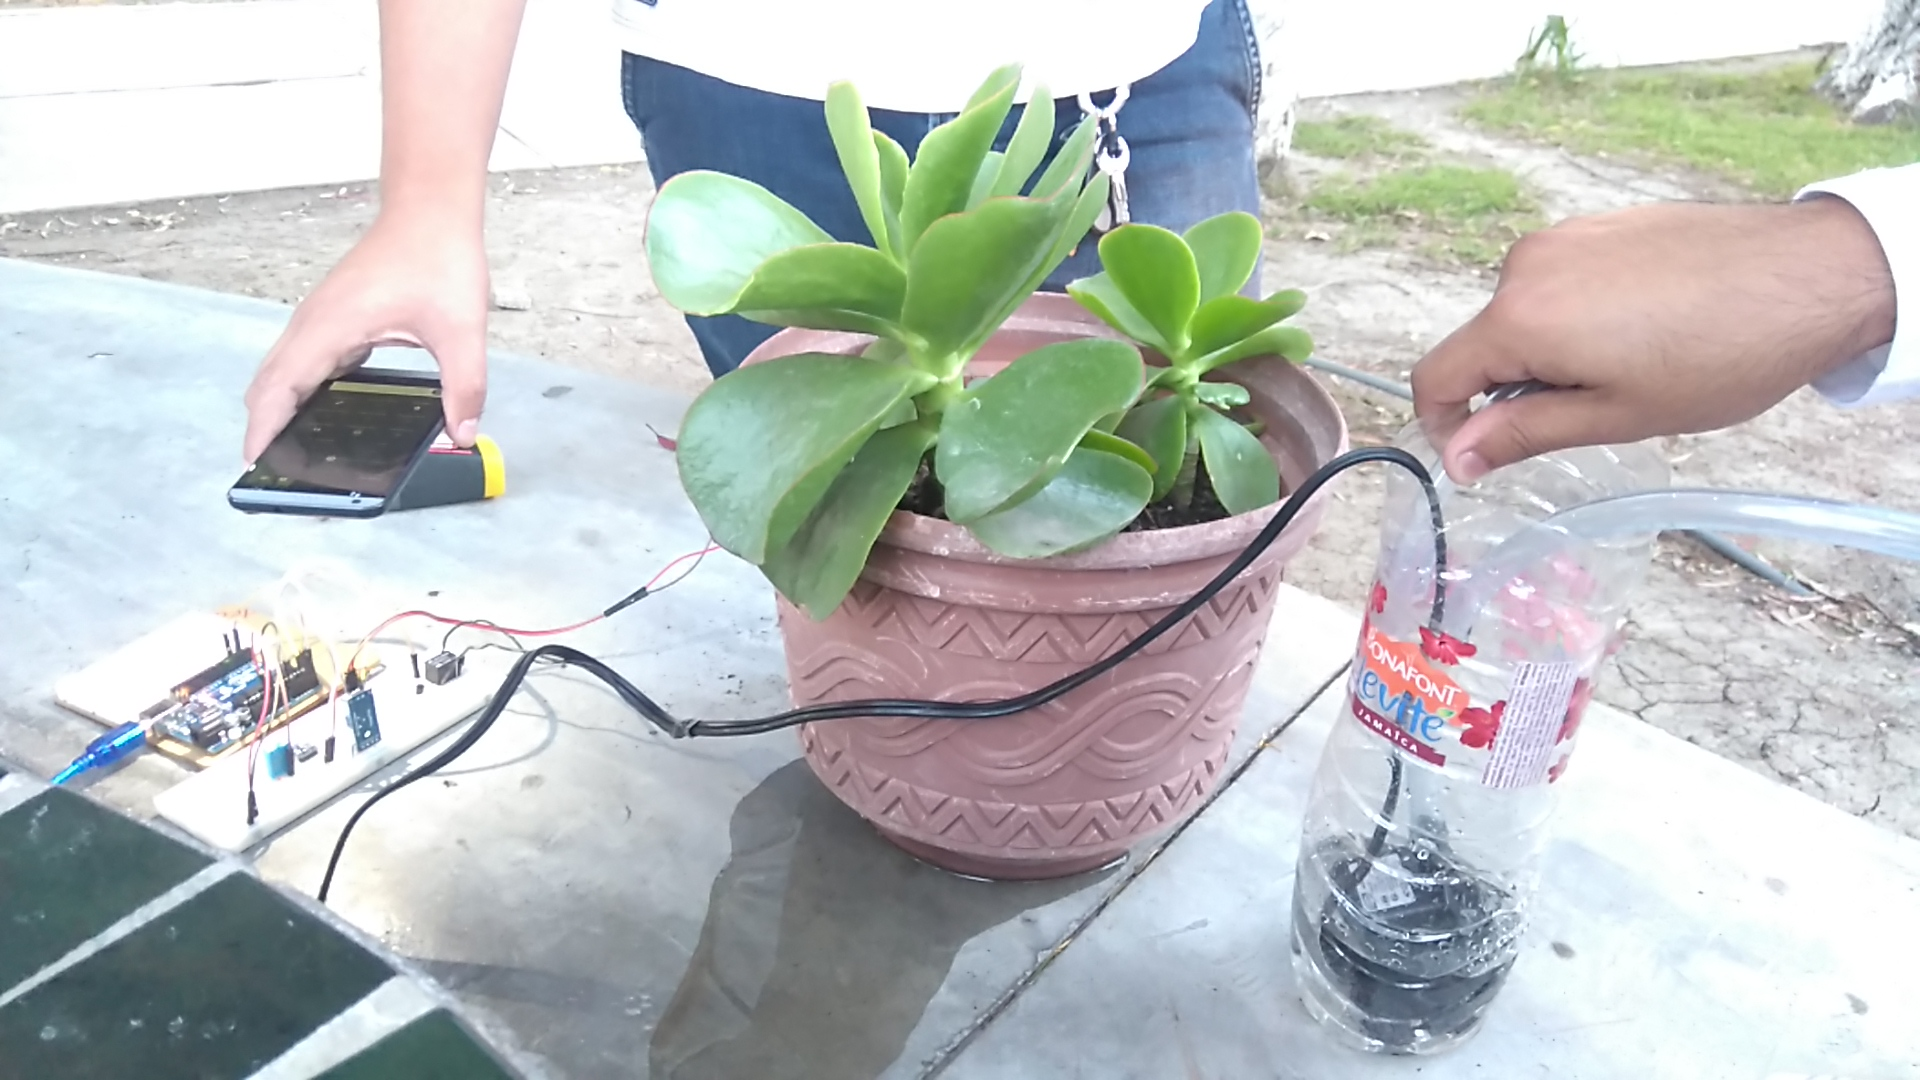
\includegraphics[width=\textwidth]{captura/1}
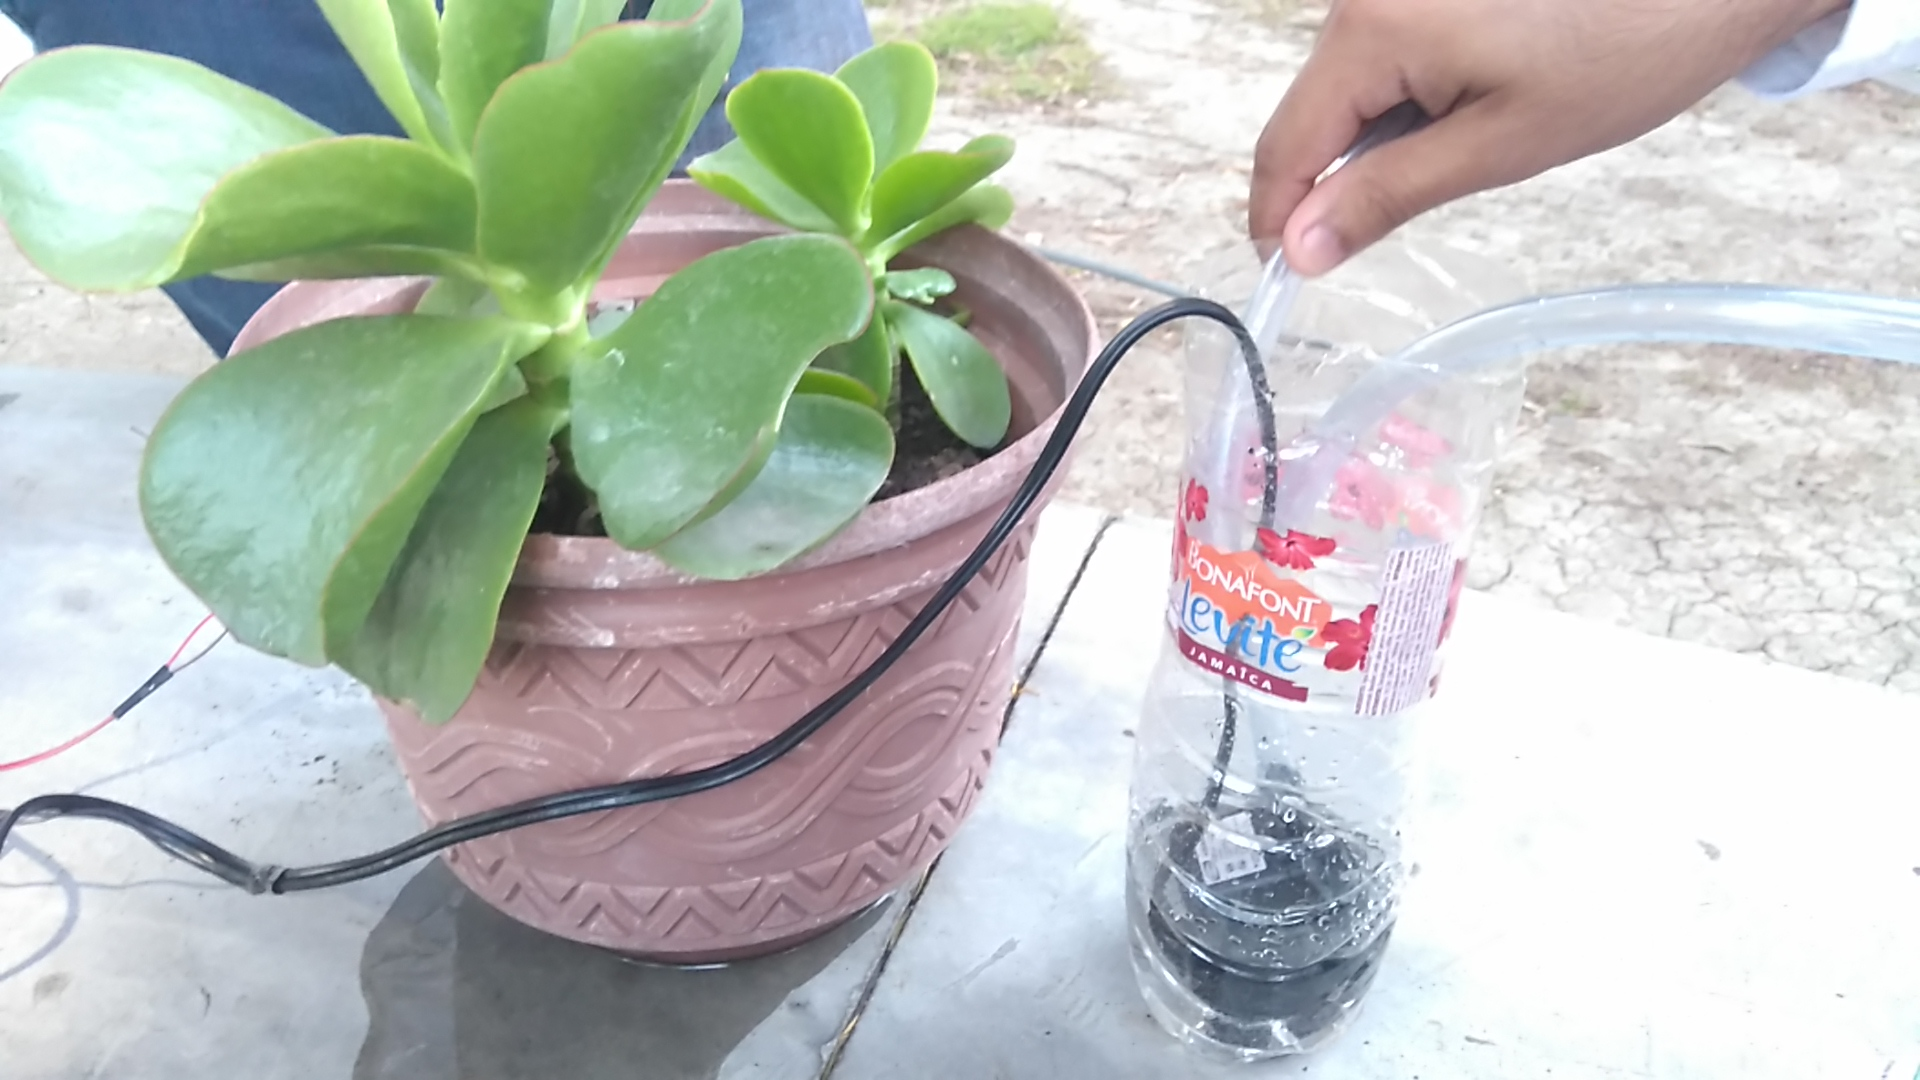
\includegraphics[width=\textwidth]{captura/2}
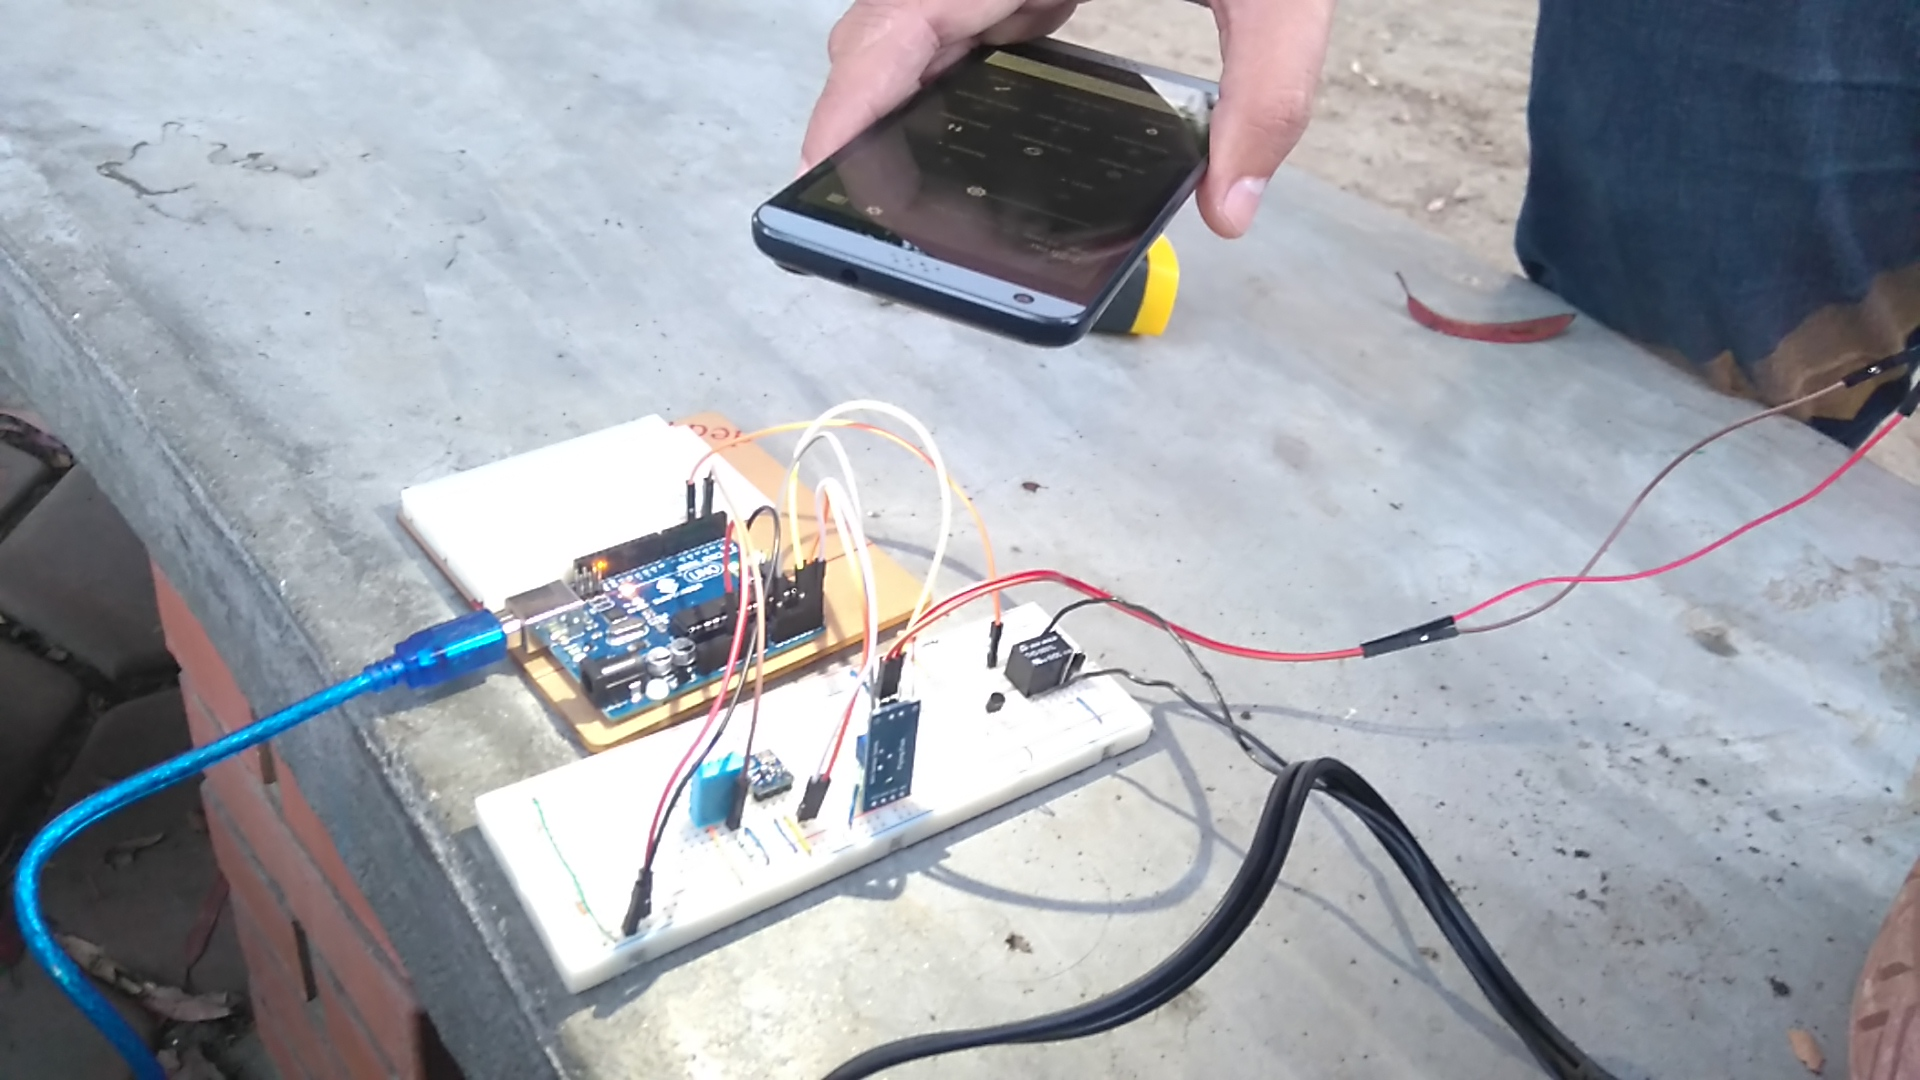
\includegraphics[width=\textwidth]{captura/3}
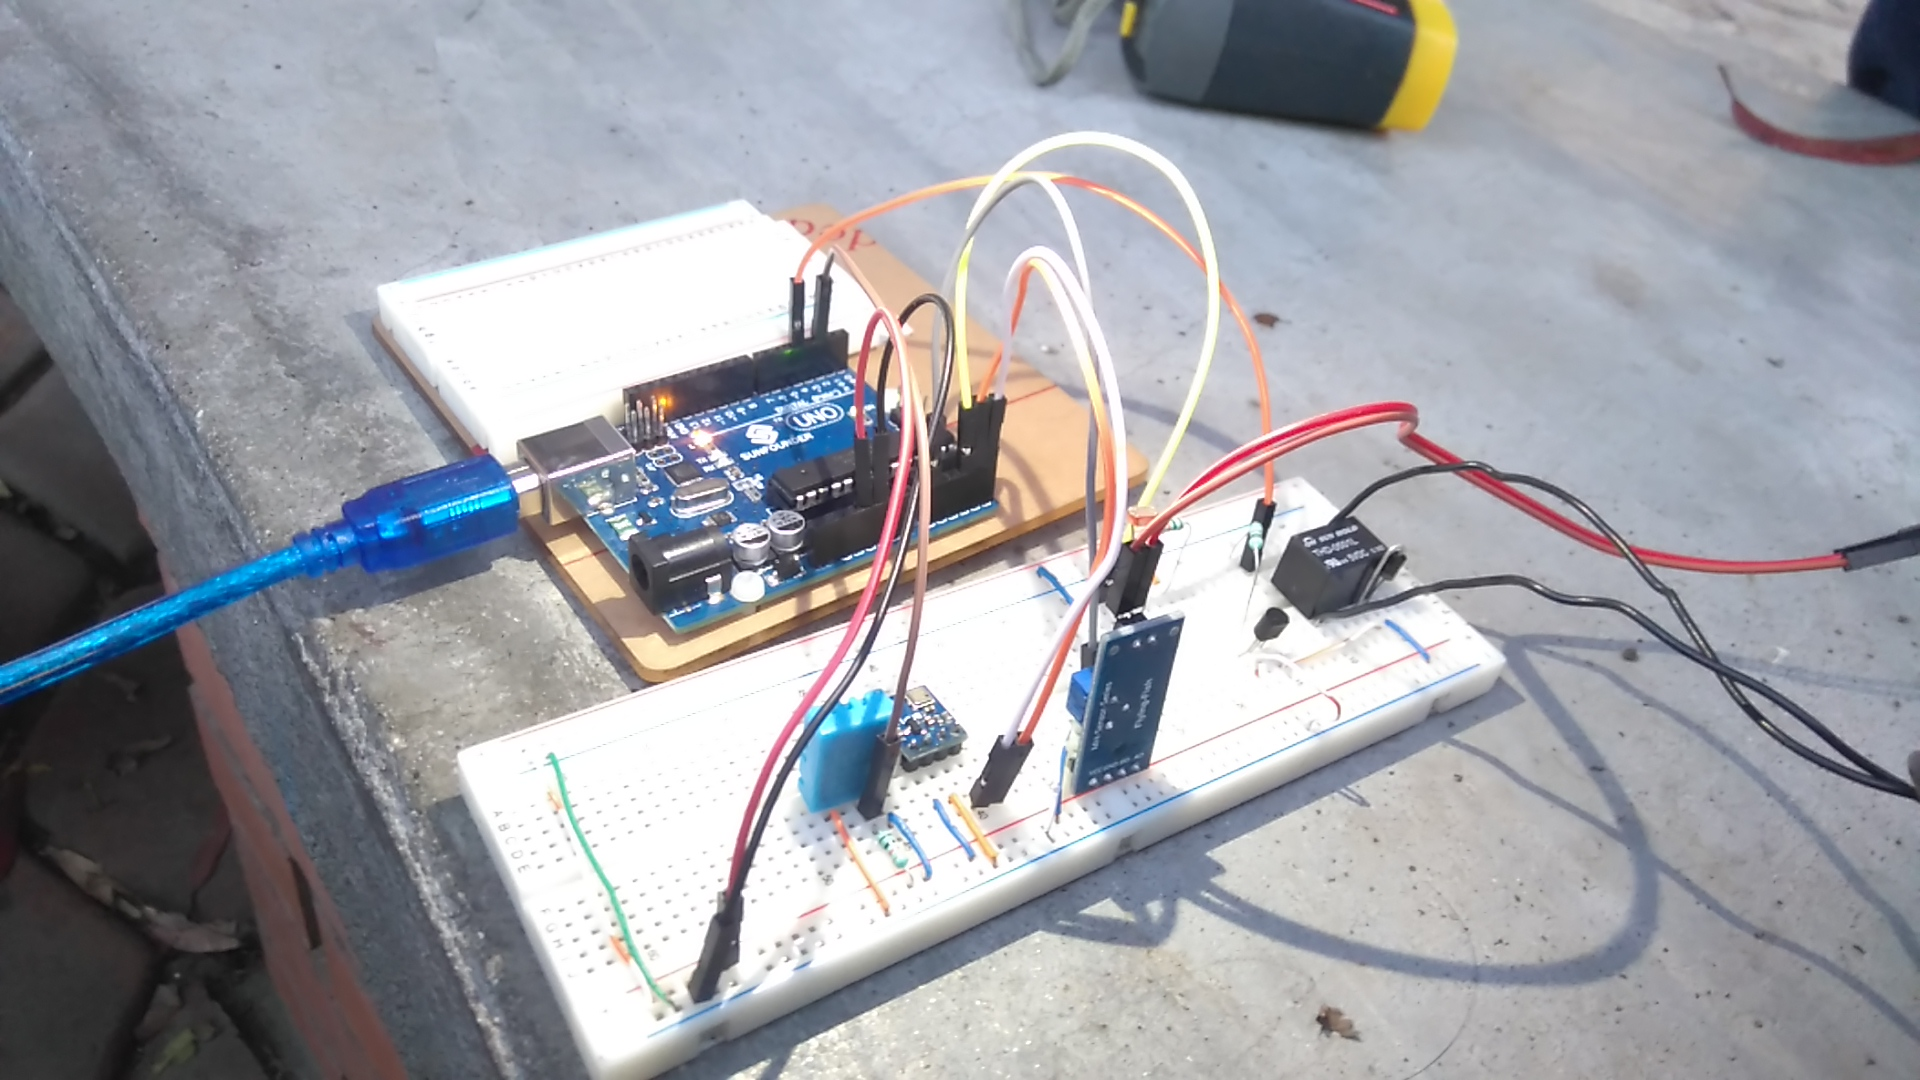
\includegraphics[width=\textwidth]{captura/4}
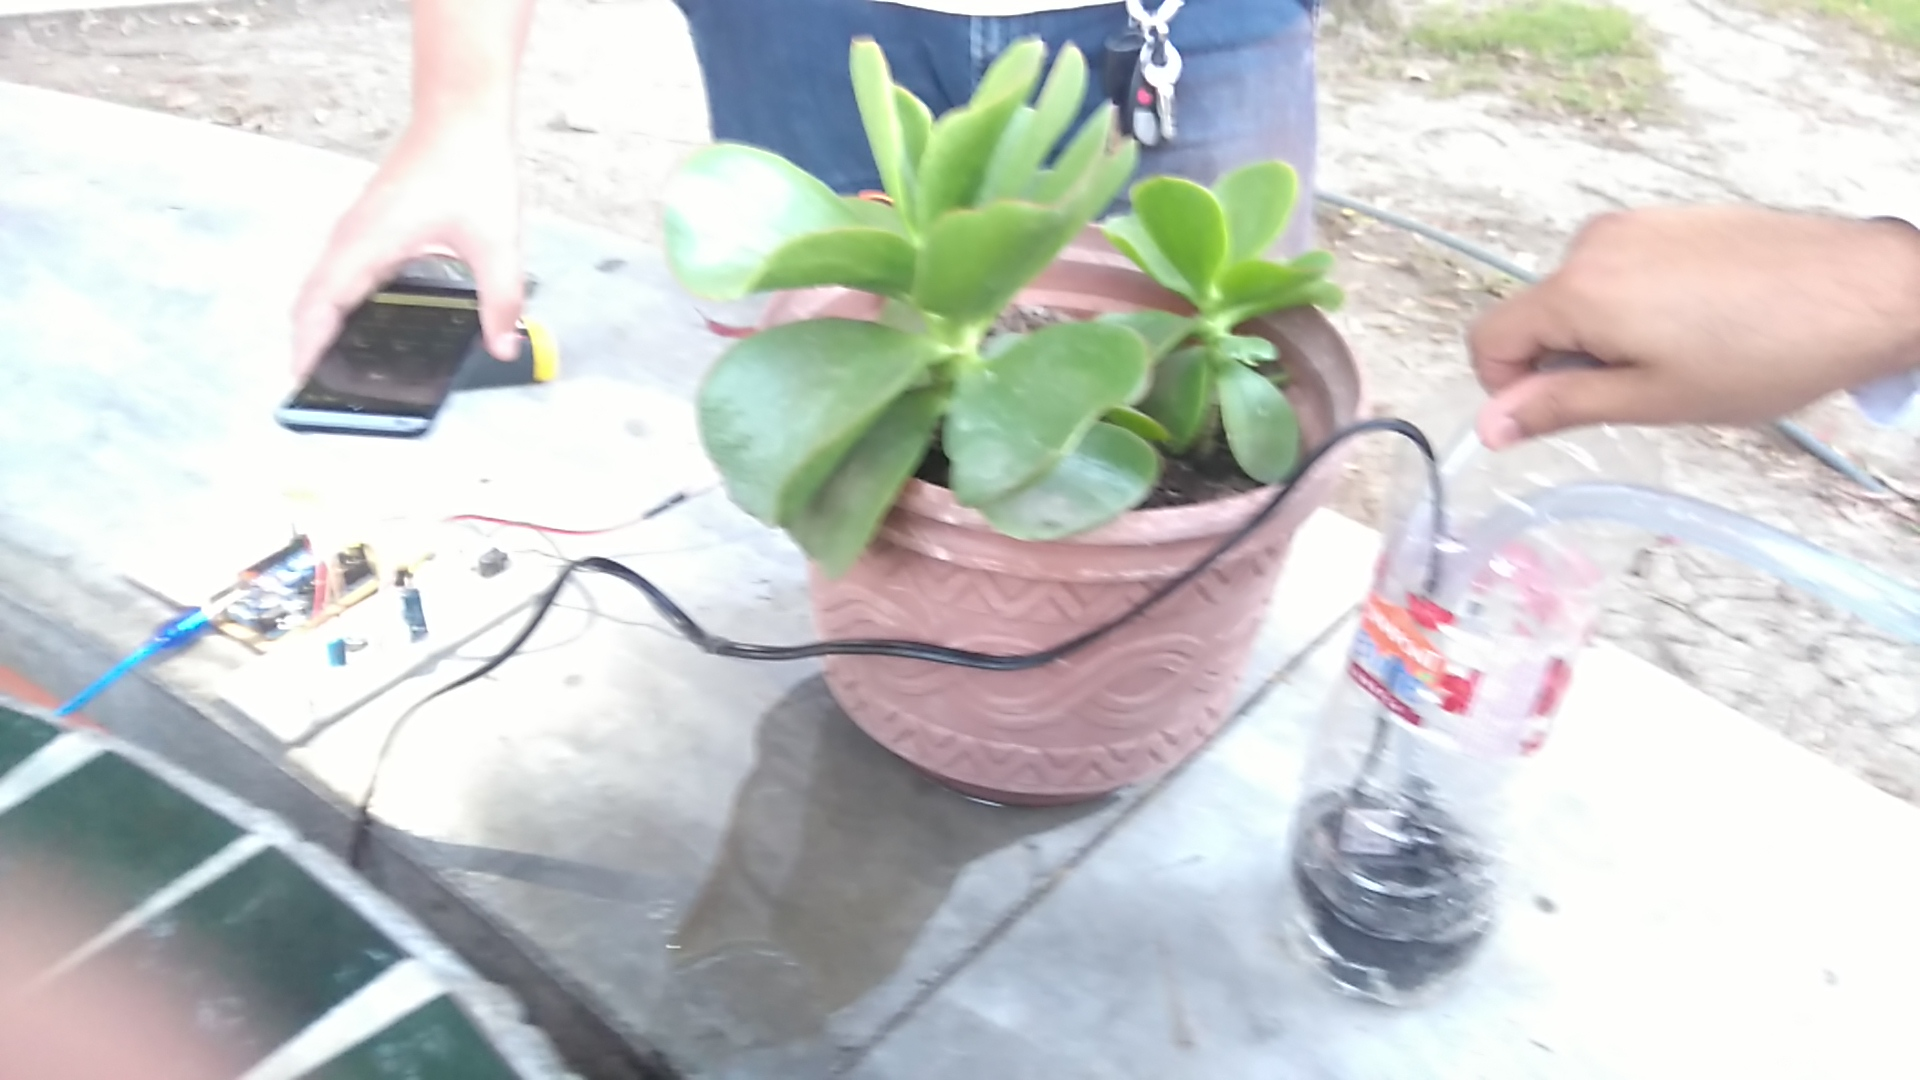
\includegraphics[width=\textwidth]{captura/5}

\newpage
\section{Conclusion}

\renewcommand\refname{Referencias}
\begin{thebibliography}{1}
	\bibitem{Arduino} What is Arduino? - Definition from Techopedia. (n.d.). Retrieved March 26, 2017, from https://www.techopedia.com/definition/27874/arduino
	\bibitem{Sensor de humedad en suelo} Electronilab from https://electronilab.co/tienda/sensor-de-humedad-de-suelo-higrometro/
	\bibitem{Sensor de humedad  y temperatura (DTH11)} HETPRO from https://hetpro-store.com/sensor-dht11-humedad/?utm\_source=google\&utm\_medium=cpc\&utm\_campaign=Product\&utm\_term=SDTH0011\&utm\_content=SDTH0011\&gclid=CjwKEAjwu4\_JBRDpgs2RwsCbt1MSJABOY8an\_YIe39bwPw9nGCoGn0nhwnEDJa0ecuyz6HhjDzsVNRoCX-7w\_wcB
	\bibitem{SensorBarometrico} BricoGeek from http://tienda.bricogeek.com/sensores/282-sensor-barometrico-bmp180.html
\end{thebibliography}

\end{document}
